\documentclass{book}
\usepackage[a4paper,top=2.5cm,bottom=2.5cm,left=2.5cm,right=2.5cm]{geometry}
\usepackage{makeidx}
\usepackage{natbib}
\usepackage{graphicx}
\usepackage{multicol}
\usepackage{float}
\usepackage{listings}
\usepackage{color}
\usepackage{ifthen}
\usepackage[table]{xcolor}
\usepackage{textcomp}
\usepackage{alltt}
\usepackage{ifpdf}
\ifpdf
\usepackage[pdftex,
            pagebackref=true,
            colorlinks=true,
            linkcolor=blue,
            unicode
           ]{hyperref}
\else
\usepackage[ps2pdf,
            pagebackref=true,
            colorlinks=true,
            linkcolor=blue,
            unicode
           ]{hyperref}
\usepackage{pspicture}
\fi
\usepackage[utf8]{inputenc}
\usepackage{mathptmx}
\usepackage[scaled=.90]{helvet}
\usepackage{courier}
\usepackage{sectsty}
\usepackage[titles]{tocloft}
\usepackage{doxygen}
\lstset{language=C++,inputencoding=utf8,basicstyle=\footnotesize,breaklines=true,breakatwhitespace=true,tabsize=8,numbers=left }
\makeindex
\setcounter{tocdepth}{3}
\renewcommand{\footrulewidth}{0.4pt}
\renewcommand{\familydefault}{\sfdefault}
\hfuzz=15pt
\setlength{\emergencystretch}{15pt}
\hbadness=750
\tolerance=750
\begin{document}
\hypersetup{pageanchor=false,citecolor=blue}
\begin{titlepage}
\vspace*{7cm}
\begin{center}
{\Large I\-U\-P\-U\-I Capstone }\\
\vspace*{1cm}
{\large Generated by Doxygen 1.8.0}\\
\vspace*{0.5cm}
{\small Sat Apr 21 2012 17:11:41}\\
\end{center}
\end{titlepage}
\clearemptydoublepage
\pagenumbering{roman}
\tableofcontents
\clearemptydoublepage
\pagenumbering{arabic}
\hypersetup{pageanchor=true,citecolor=blue}
\chapter{Class Index}
\section{Class Hierarchy}
This inheritance list is sorted roughly, but not completely, alphabetically\-:\begin{DoxyCompactList}
\item \contentsline{section}{Arduino\-Interface.\-Arduino\-Interface}{\pageref{class_arduino_interface_1_1_arduino_interface}}{}
\item \contentsline{section}{Database\-Interface.\-Database\-Interface}{\pageref{class_database_interface_1_1_database_interface}}{}
\begin{DoxyCompactList}
\item \contentsline{section}{Dump\-To\-Remote.\-Dump\-To\-Remote}{\pageref{class_dump_to_remote_1_1_dump_to_remote}}{}
\item \contentsline{section}{Fill\-Data.\-Fill\-Data}{\pageref{class_fill_data_1_1_fill_data}}{}
\end{DoxyCompactList}
\item \contentsline{section}{Error.\-Error}{\pageref{class_error_1_1_error}}{}
\begin{DoxyCompactList}
\item \contentsline{section}{Error.\-arduino\-Error}{\pageref{class_error_1_1arduino_error}}{}
\item \contentsline{section}{Error.\-My\-Error}{\pageref{class_error_1_1_my_error}}{}
\end{DoxyCompactList}
\item \contentsline{section}{Gui\-Interface.\-gui\-Interface}{\pageref{class_gui_interface_1_1gui_interface}}{}
\end{DoxyCompactList}

\chapter{Class Index}
\section{Class List}
Here are the classes, structs, unions and interfaces with brief descriptions\-:\begin{DoxyCompactList}
\item\contentsline{section}{\hyperlink{class_error_1_1arduino_error}{Error.\-arduino\-Error} }{\pageref{class_error_1_1arduino_error}}{}
\item\contentsline{section}{\hyperlink{class_arduino_interface_1_1_arduino_interface}{Arduino\-Interface.\-Arduino\-Interface} }{\pageref{class_arduino_interface_1_1_arduino_interface}}{}
\item\contentsline{section}{\hyperlink{class_database_interface_1_1_database_interface}{Database\-Interface.\-Database\-Interface} }{\pageref{class_database_interface_1_1_database_interface}}{}
\item\contentsline{section}{\hyperlink{class_dump_to_remote_1_1_dump_to_remote}{Dump\-To\-Remote.\-Dump\-To\-Remote} }{\pageref{class_dump_to_remote_1_1_dump_to_remote}}{}
\item\contentsline{section}{\hyperlink{class_error_1_1_error}{Error.\-Error} }{\pageref{class_error_1_1_error}}{}
\item\contentsline{section}{\hyperlink{class_fill_data_1_1_fill_data}{Fill\-Data.\-Fill\-Data} }{\pageref{class_fill_data_1_1_fill_data}}{}
\item\contentsline{section}{\hyperlink{class_gui_interface_1_1gui_interface}{Gui\-Interface.\-gui\-Interface} }{\pageref{class_gui_interface_1_1gui_interface}}{}
\item\contentsline{section}{\hyperlink{class_error_1_1_my_error}{Error.\-My\-Error} }{\pageref{class_error_1_1_my_error}}{}
\end{DoxyCompactList}

\chapter{Class Documentation}
\hypertarget{class_error_1_1arduino_error}{\section{Error.\-arduino\-Error Class Reference}
\label{class_error_1_1arduino_error}\index{Error.\-arduino\-Error@{Error.\-arduino\-Error}}
}
Inheritance diagram for Error.\-arduino\-Error\-:\begin{figure}[H]
\begin{center}
\leavevmode
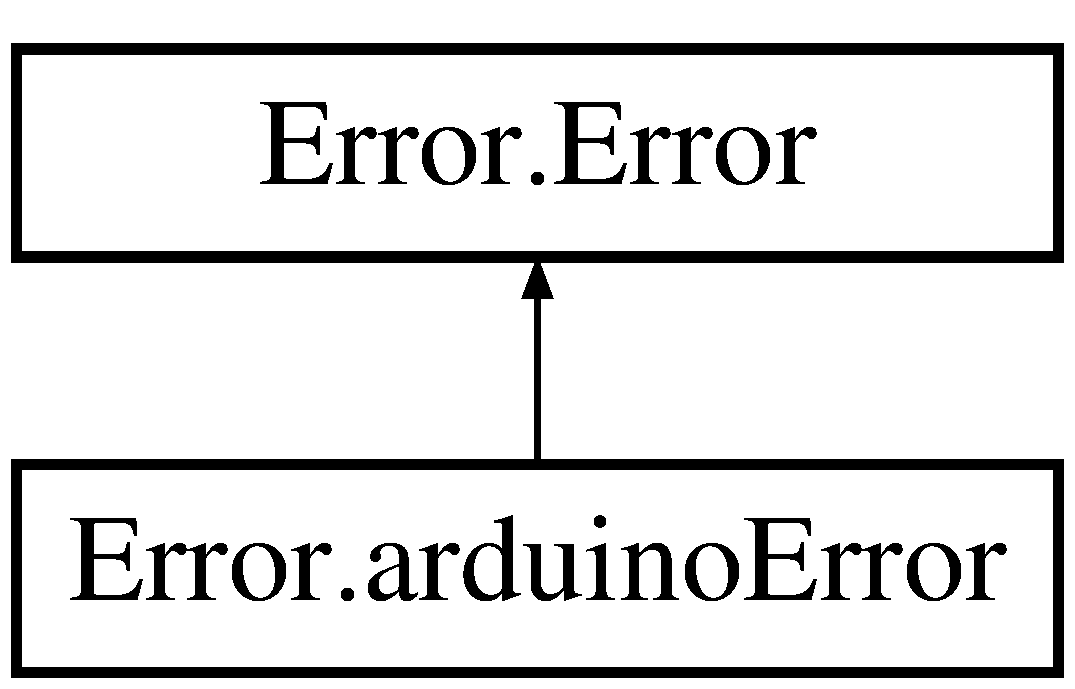
\includegraphics[height=2.000000cm]{class_error_1_1arduino_error}
\end{center}
\end{figure}
\subsection*{Public Member Functions}
\begin{DoxyCompactItemize}
\item 
def \hyperlink{class_error_1_1arduino_error_af4c491b29579c8b181813815e7e8914b}{\-\_\-\-\_\-init\-\_\-\-\_\-}
\end{DoxyCompactItemize}
\subsection*{Public Attributes}
\begin{DoxyCompactItemize}
\item 
\hyperlink{class_error_1_1arduino_error_abd38cfdb82bda4f911c41d018130a3d0}{expr}
\item 
\hyperlink{class_error_1_1arduino_error_aa963133e309f1c2240e98e81d9c092e0}{msg}
\end{DoxyCompactItemize}


\subsection{Constructor \& Destructor Documentation}
\hypertarget{class_error_1_1arduino_error_af4c491b29579c8b181813815e7e8914b}{\index{Error\-::arduino\-Error@{Error\-::arduino\-Error}!\-\_\-\-\_\-init\-\_\-\-\_\-@{\-\_\-\-\_\-init\-\_\-\-\_\-}}
\index{\-\_\-\-\_\-init\-\_\-\-\_\-@{\-\_\-\-\_\-init\-\_\-\-\_\-}!Error::arduinoError@{Error\-::arduino\-Error}}
\subsubsection[{\-\_\-\-\_\-init\-\_\-\-\_\-}]{\setlength{\rightskip}{0pt plus 5cm}def {\bf Error.\-arduino\-Error.\-\_\-\-\_\-init\-\_\-\-\_\-} (
\begin{DoxyParamCaption}
\item[{}]{self, }
\item[{}]{expr, }
\item[{}]{msg}
\end{DoxyParamCaption}
)}}\label{class_error_1_1arduino_error_af4c491b29579c8b181813815e7e8914b}


\subsection{Member Data Documentation}
\hypertarget{class_error_1_1arduino_error_abd38cfdb82bda4f911c41d018130a3d0}{\index{Error\-::arduino\-Error@{Error\-::arduino\-Error}!expr@{expr}}
\index{expr@{expr}!Error::arduinoError@{Error\-::arduino\-Error}}
\subsubsection[{expr}]{\setlength{\rightskip}{0pt plus 5cm}{\bf Error.\-arduino\-Error.\-expr}}}\label{class_error_1_1arduino_error_abd38cfdb82bda4f911c41d018130a3d0}
\hypertarget{class_error_1_1arduino_error_aa963133e309f1c2240e98e81d9c092e0}{\index{Error\-::arduino\-Error@{Error\-::arduino\-Error}!msg@{msg}}
\index{msg@{msg}!Error::arduinoError@{Error\-::arduino\-Error}}
\subsubsection[{msg}]{\setlength{\rightskip}{0pt plus 5cm}{\bf Error.\-arduino\-Error.\-msg}}}\label{class_error_1_1arduino_error_aa963133e309f1c2240e98e81d9c092e0}


The documentation for this class was generated from the following file\-:\begin{DoxyCompactItemize}
\item 
A\-:/documents/nathan/\-My Documents/\-Dropbox/\-Workspace/spring2012/\-C\-S495/code/\-Airqual\-Repo/air\-\_\-quality/python\-\_\-src/\hyperlink{_error_8py}{Error.\-py}\end{DoxyCompactItemize}

\hypertarget{class_arduino_interface_1_1_arduino_interface}{\section{Arduino\-Interface.\-Arduino\-Interface Class Reference}
\label{class_arduino_interface_1_1_arduino_interface}\index{Arduino\-Interface.\-Arduino\-Interface@{Arduino\-Interface.\-Arduino\-Interface}}
}
\subsection*{Public Member Functions}
\begin{DoxyCompactItemize}
\item 
\hypertarget{class_arduino_interface_1_1_arduino_interface_ad0063b90161fa8323cef433a13bb6e8b}{def {\bfseries \-\_\-\-\_\-init\-\_\-\-\_\-}}\label{class_arduino_interface_1_1_arduino_interface_ad0063b90161fa8323cef433a13bb6e8b}

\item 
\hypertarget{class_arduino_interface_1_1_arduino_interface_aa292ce6b4406b3e975e703502cca0e39}{def {\bfseries send\-Data}}\label{class_arduino_interface_1_1_arduino_interface_aa292ce6b4406b3e975e703502cca0e39}

\item 
\hypertarget{class_arduino_interface_1_1_arduino_interface_ae1ac3ad21ffe702a7b97ac3e05a22fc0}{def {\bfseries get\-Data}}\label{class_arduino_interface_1_1_arduino_interface_ae1ac3ad21ffe702a7b97ac3e05a22fc0}

\item 
\hypertarget{class_arduino_interface_1_1_arduino_interface_af07f9f858c6274d9cc1247c7dd14ebf6}{def {\bfseries print\-Serial}}\label{class_arduino_interface_1_1_arduino_interface_af07f9f858c6274d9cc1247c7dd14ebf6}

\item 
\hypertarget{class_arduino_interface_1_1_arduino_interface_a0e311cf3263799415c2ff536c7b42cf8}{def {\bfseries get\-Connection}}\label{class_arduino_interface_1_1_arduino_interface_a0e311cf3263799415c2ff536c7b42cf8}

\item 
\hypertarget{class_arduino_interface_1_1_arduino_interface_ac215fb8000c089a566d70f1b59c272b3}{def {\bfseries main}}\label{class_arduino_interface_1_1_arduino_interface_ac215fb8000c089a566d70f1b59c272b3}

\end{DoxyCompactItemize}


The documentation for this class was generated from the following file\-:\begin{DoxyCompactItemize}
\item 
C\-:/\-Users/nathan.\-boyd/\-Dropbox/\-Workspace/spring2012/\-C\-S495/code/\-Airqual\-Repo/air\-\_\-quality/python\-\_\-src/Arduino\-Interface.\-py\end{DoxyCompactItemize}

\hypertarget{class_database_interface_1_1_database_interface}{\section{Database\-Interface.\-Database\-Interface Class Reference}
\label{class_database_interface_1_1_database_interface}\index{Database\-Interface.\-Database\-Interface@{Database\-Interface.\-Database\-Interface}}
}
Inheritance diagram for Database\-Interface.\-Database\-Interface\-:\begin{figure}[H]
\begin{center}
\leavevmode
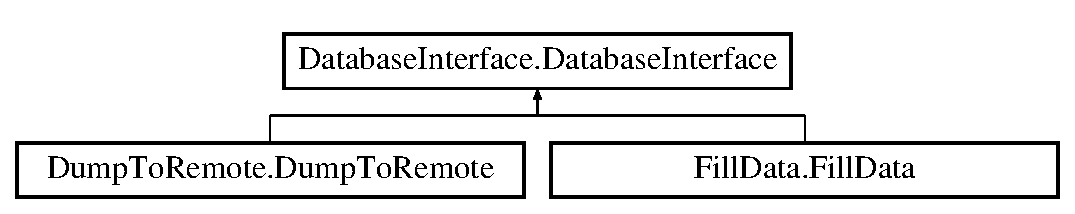
\includegraphics[height=2.000000cm]{class_database_interface_1_1_database_interface}
\end{center}
\end{figure}
\subsection*{Public Member Functions}
\begin{DoxyCompactItemize}
\item 
\hypertarget{class_database_interface_1_1_database_interface_a79b2f185cf35d225238e22921254ba0f}{def {\bfseries \-\_\-\-\_\-init\-\_\-\-\_\-}}\label{class_database_interface_1_1_database_interface_a79b2f185cf35d225238e22921254ba0f}

\item 
\hypertarget{class_database_interface_1_1_database_interface_a9c7a69525645d39f1d2967b2221b0e95}{def {\bfseries get\-Cursor}}\label{class_database_interface_1_1_database_interface_a9c7a69525645d39f1d2967b2221b0e95}

\item 
\hypertarget{class_database_interface_1_1_database_interface_a403157af3a4e682ce0244a59885980e3}{def {\bfseries create\-Table}}\label{class_database_interface_1_1_database_interface_a403157af3a4e682ce0244a59885980e3}

\item 
\hypertarget{class_database_interface_1_1_database_interface_a0cdcada6026e9de3ef363e7ffe43a055}{def {\bfseries table\-Exists}}\label{class_database_interface_1_1_database_interface_a0cdcada6026e9de3ef363e7ffe43a055}

\item 
\hypertarget{class_database_interface_1_1_database_interface_a62f0ccdb9b87ae7fd37f57058177b29b}{def {\bfseries insert\-Data\-Point}}\label{class_database_interface_1_1_database_interface_a62f0ccdb9b87ae7fd37f57058177b29b}

\item 
\hypertarget{class_database_interface_1_1_database_interface_a5ce1c3e2d2da9cfc3e51162f8ce00e63}{def {\bfseries insert\-Row}}\label{class_database_interface_1_1_database_interface_a5ce1c3e2d2da9cfc3e51162f8ce00e63}

\item 
\hypertarget{class_database_interface_1_1_database_interface_a34cd488b227a7742298c622a70511ae1}{def {\bfseries main}}\label{class_database_interface_1_1_database_interface_a34cd488b227a7742298c622a70511ae1}

\end{DoxyCompactItemize}
\subsection*{Static Public Attributes}
\begin{DoxyCompactItemize}
\item 
\hypertarget{class_database_interface_1_1_database_interface_ac0a2837d86558a1bfe62834dcd6274f3}{string {\bfseries W\-O\-R\-K\-I\-N\-G\-\_\-\-D\-B} = 'local'}\label{class_database_interface_1_1_database_interface_ac0a2837d86558a1bfe62834dcd6274f3}

\item 
\hypertarget{class_database_interface_1_1_database_interface_ae92289621f90ec296eb0cd89b9f6fc91}{{\bfseries D\-E\-B\-U\-G} = False}\label{class_database_interface_1_1_database_interface_ae92289621f90ec296eb0cd89b9f6fc91}

\end{DoxyCompactItemize}


The documentation for this class was generated from the following file\-:\begin{DoxyCompactItemize}
\item 
C\-:/\-Users/nathan.\-boyd/\-Dropbox/\-Workspace/spring2012/\-C\-S495/code/\-Airqual\-Repo/air\-\_\-quality/python\-\_\-src/Database\-Interface.\-py\end{DoxyCompactItemize}

\hypertarget{class_dump_to_remote_1_1_dump_to_remote}{\section{Dump\-To\-Remote.\-Dump\-To\-Remote Class Reference}
\label{class_dump_to_remote_1_1_dump_to_remote}\index{Dump\-To\-Remote.\-Dump\-To\-Remote@{Dump\-To\-Remote.\-Dump\-To\-Remote}}
}
Inheritance diagram for Dump\-To\-Remote.\-Dump\-To\-Remote\-:\begin{figure}[H]
\begin{center}
\leavevmode
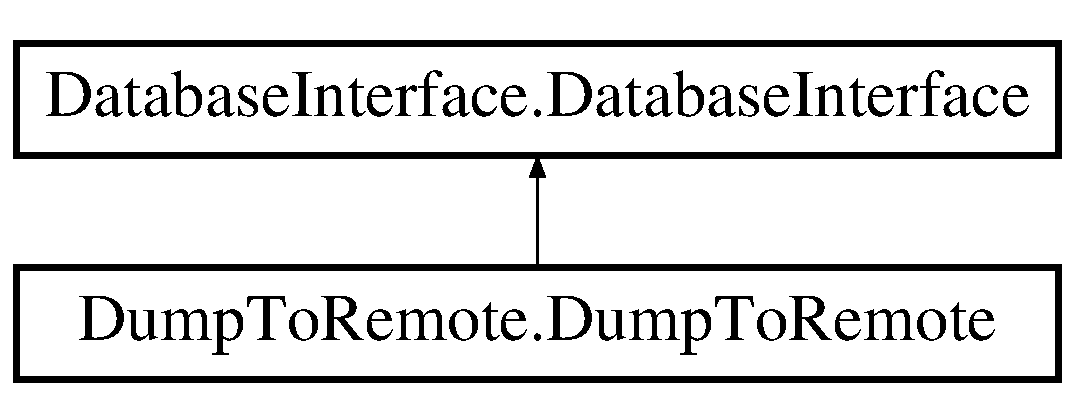
\includegraphics[height=2.000000cm]{class_dump_to_remote_1_1_dump_to_remote}
\end{center}
\end{figure}
\subsection*{Public Member Functions}
\begin{DoxyCompactItemize}
\item 
\hypertarget{class_dump_to_remote_1_1_dump_to_remote_ad564941589b93a68ff46498cc21da2f2}{def {\bfseries \-\_\-\-\_\-init\-\_\-\-\_\-}}\label{class_dump_to_remote_1_1_dump_to_remote_ad564941589b93a68ff46498cc21da2f2}

\item 
\hypertarget{class_dump_to_remote_1_1_dump_to_remote_adb91f51d25a482426704c6a0c0c1377f}{def {\bfseries main}}\label{class_dump_to_remote_1_1_dump_to_remote_adb91f51d25a482426704c6a0c0c1377f}

\end{DoxyCompactItemize}


The documentation for this class was generated from the following file\-:\begin{DoxyCompactItemize}
\item 
C\-:/\-Users/nathan.\-boyd/\-Dropbox/\-Workspace/spring2012/\-C\-S495/code/\-Airqual\-Repo/air\-\_\-quality/python\-\_\-src/Dump\-To\-Remote.\-py\end{DoxyCompactItemize}

\hypertarget{class_error_1_1_error}{\section{Error.\-Error Class Reference}
\label{class_error_1_1_error}\index{Error.\-Error@{Error.\-Error}}
}
Inheritance diagram for Error.\-Error\-:\begin{figure}[H]
\begin{center}
\leavevmode
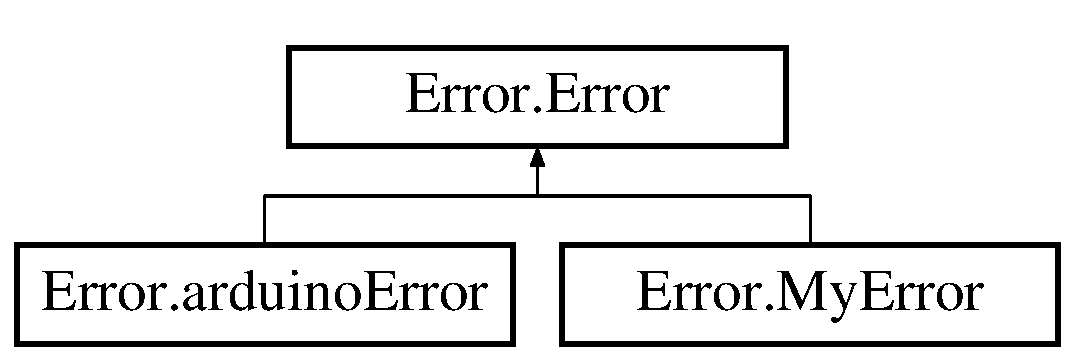
\includegraphics[height=2.000000cm]{class_error_1_1_error}
\end{center}
\end{figure}


\subsection{Detailed Description}
\begin{DoxyVerb}Base class for exceptions in this module.\end{DoxyVerb}
 

The documentation for this class was generated from the following file\-:\begin{DoxyCompactItemize}
\item 
A\-:/documents/nathan/\-My Documents/\-Dropbox/\-Workspace/spring2012/\-C\-S495/code/\-Airqual\-Repo/air\-\_\-quality/python\-\_\-src/\hyperlink{_error_8py}{Error.\-py}\end{DoxyCompactItemize}

\hypertarget{class_fill_data_1_1_fill_data}{\section{Fill\-Data.\-Fill\-Data Class Reference}
\label{class_fill_data_1_1_fill_data}\index{Fill\-Data.\-Fill\-Data@{Fill\-Data.\-Fill\-Data}}
}
Inheritance diagram for Fill\-Data.\-Fill\-Data\-:\begin{figure}[H]
\begin{center}
\leavevmode
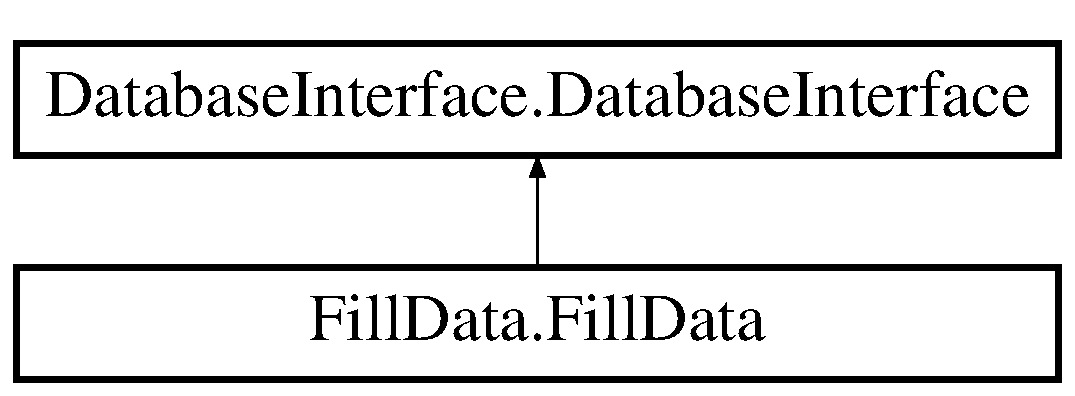
\includegraphics[height=2.000000cm]{class_fill_data_1_1_fill_data}
\end{center}
\end{figure}
\subsection*{Public Member Functions}
\begin{DoxyCompactItemize}
\item 
\hypertarget{class_fill_data_1_1_fill_data_af740b6816f2b16d11688251cbd0eefff}{def {\bfseries \-\_\-\-\_\-init\-\_\-\-\_\-}}\label{class_fill_data_1_1_fill_data_af740b6816f2b16d11688251cbd0eefff}

\item 
\hypertarget{class_fill_data_1_1_fill_data_acce1c8c84567e2e1cf45e0160d80006e}{def {\bfseries check\-Townships}}\label{class_fill_data_1_1_fill_data_acce1c8c84567e2e1cf45e0160d80006e}

\item 
\hypertarget{class_fill_data_1_1_fill_data_af9c92e35e375bed232be9bec5bce5ad0}{def {\bfseries check\-Addresses}}\label{class_fill_data_1_1_fill_data_af9c92e35e375bed232be9bec5bce5ad0}

\item 
\hypertarget{class_fill_data_1_1_fill_data_a8a24290464e37b6f668338c7b75dab69}{def {\bfseries main}}\label{class_fill_data_1_1_fill_data_a8a24290464e37b6f668338c7b75dab69}

\end{DoxyCompactItemize}


The documentation for this class was generated from the following file\-:\begin{DoxyCompactItemize}
\item 
C\-:/\-Users/nathan.\-boyd/\-Dropbox/\-Workspace/spring2012/\-C\-S495/code/\-Airqual\-Repo/air\-\_\-quality/python\-\_\-src/Fill\-Data.\-py\end{DoxyCompactItemize}

\hypertarget{class_gui_interface_1_1gui_interface}{\section{Gui\-Interface.\-gui\-Interface Class Reference}
\label{class_gui_interface_1_1gui_interface}\index{Gui\-Interface.\-gui\-Interface@{Gui\-Interface.\-gui\-Interface}}
}
\subsection*{Public Member Functions}
\begin{DoxyCompactItemize}
\item 
def \hyperlink{class_gui_interface_1_1gui_interface_ac54648b04404d73cdf5cc648cd0df814}{start\-Sensor}
\item 
def \hyperlink{class_gui_interface_1_1gui_interface_a87f803203fddf02263f7edf07e47097a}{fill\-Locality}
\item 
def \hyperlink{class_gui_interface_1_1gui_interface_a64d4c8bc5d86f421303bddf0d12d18f3}{dump\-To\-Remote}
\item 
def \hyperlink{class_gui_interface_1_1gui_interface_a57f43b82011bb65e63628118e023b748}{main}
\end{DoxyCompactItemize}


\subsection{Member Function Documentation}
\hypertarget{class_gui_interface_1_1gui_interface_a64d4c8bc5d86f421303bddf0d12d18f3}{\index{Gui\-Interface\-::gui\-Interface@{Gui\-Interface\-::gui\-Interface}!dump\-To\-Remote@{dump\-To\-Remote}}
\index{dump\-To\-Remote@{dump\-To\-Remote}!GuiInterface::guiInterface@{Gui\-Interface\-::gui\-Interface}}
\subsubsection[{dump\-To\-Remote}]{\setlength{\rightskip}{0pt plus 5cm}def {\bf Gui\-Interface.\-gui\-Interface.\-dump\-To\-Remote} (
\begin{DoxyParamCaption}
\item[{}]{self}
\end{DoxyParamCaption}
)}}\label{class_gui_interface_1_1gui_interface_a64d4c8bc5d86f421303bddf0d12d18f3}
\hypertarget{class_gui_interface_1_1gui_interface_a87f803203fddf02263f7edf07e47097a}{\index{Gui\-Interface\-::gui\-Interface@{Gui\-Interface\-::gui\-Interface}!fill\-Locality@{fill\-Locality}}
\index{fill\-Locality@{fill\-Locality}!GuiInterface::guiInterface@{Gui\-Interface\-::gui\-Interface}}
\subsubsection[{fill\-Locality}]{\setlength{\rightskip}{0pt plus 5cm}def {\bf Gui\-Interface.\-gui\-Interface.\-fill\-Locality} (
\begin{DoxyParamCaption}
\item[{}]{self}
\end{DoxyParamCaption}
)}}\label{class_gui_interface_1_1gui_interface_a87f803203fddf02263f7edf07e47097a}
\hypertarget{class_gui_interface_1_1gui_interface_a57f43b82011bb65e63628118e023b748}{\index{Gui\-Interface\-::gui\-Interface@{Gui\-Interface\-::gui\-Interface}!main@{main}}
\index{main@{main}!GuiInterface::guiInterface@{Gui\-Interface\-::gui\-Interface}}
\subsubsection[{main}]{\setlength{\rightskip}{0pt plus 5cm}def {\bf Gui\-Interface.\-gui\-Interface.\-main} (
\begin{DoxyParamCaption}
\item[{}]{self}
\end{DoxyParamCaption}
)}}\label{class_gui_interface_1_1gui_interface_a57f43b82011bb65e63628118e023b748}
\hypertarget{class_gui_interface_1_1gui_interface_ac54648b04404d73cdf5cc648cd0df814}{\index{Gui\-Interface\-::gui\-Interface@{Gui\-Interface\-::gui\-Interface}!start\-Sensor@{start\-Sensor}}
\index{start\-Sensor@{start\-Sensor}!GuiInterface::guiInterface@{Gui\-Interface\-::gui\-Interface}}
\subsubsection[{start\-Sensor}]{\setlength{\rightskip}{0pt plus 5cm}def {\bf Gui\-Interface.\-gui\-Interface.\-start\-Sensor} (
\begin{DoxyParamCaption}
\item[{}]{self}
\end{DoxyParamCaption}
)}}\label{class_gui_interface_1_1gui_interface_ac54648b04404d73cdf5cc648cd0df814}


The documentation for this class was generated from the following file\-:\begin{DoxyCompactItemize}
\item 
A\-:/documents/nathan/\-My Documents/\-Dropbox/\-Workspace/spring2012/\-C\-S495/code/\-Airqual\-Repo/air\-\_\-quality/python\-\_\-src/\hyperlink{_gui_interface_8py}{Gui\-Interface.\-py}\end{DoxyCompactItemize}

\hypertarget{class_error_1_1_my_error}{\section{Error.\-My\-Error Class Reference}
\label{class_error_1_1_my_error}\index{Error.\-My\-Error@{Error.\-My\-Error}}
}
Inheritance diagram for Error.\-My\-Error\-:\begin{figure}[H]
\begin{center}
\leavevmode
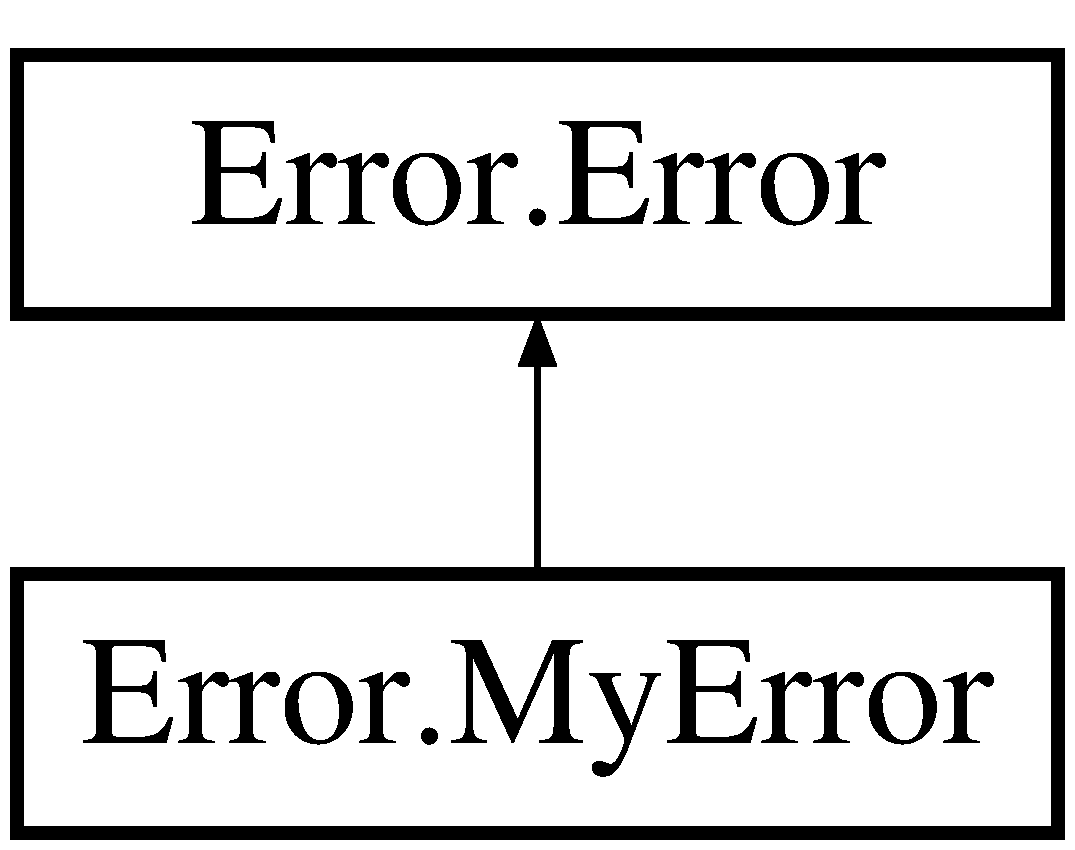
\includegraphics[height=2.000000cm]{class_error_1_1_my_error}
\end{center}
\end{figure}
\subsection*{Public Member Functions}
\begin{DoxyCompactItemize}
\item 
\hypertarget{class_error_1_1_my_error_a7a269ccbf9182b2a818d1a33c0436bce}{def {\bfseries \-\_\-\-\_\-init\-\_\-\-\_\-}}\label{class_error_1_1_my_error_a7a269ccbf9182b2a818d1a33c0436bce}

\item 
\hypertarget{class_error_1_1_my_error_a7ce4fb2ab3d7e6ef6a393c4e09c99618}{def {\bfseries \-\_\-\-\_\-str\-\_\-\-\_\-}}\label{class_error_1_1_my_error_a7ce4fb2ab3d7e6ef6a393c4e09c99618}

\end{DoxyCompactItemize}
\subsection*{Public Attributes}
\begin{DoxyCompactItemize}
\item 
\hypertarget{class_error_1_1_my_error_a768d5e180ecca5aaf742c1389dcfeb00}{{\bfseries value}}\label{class_error_1_1_my_error_a768d5e180ecca5aaf742c1389dcfeb00}

\end{DoxyCompactItemize}


The documentation for this class was generated from the following file\-:\begin{DoxyCompactItemize}
\item 
C\-:/\-Users/nathan.\-boyd/\-Dropbox/\-Workspace/spring2012/\-C\-S495/code/\-Airqual\-Repo/air\-\_\-quality/python\-\_\-src/Error.\-py\end{DoxyCompactItemize}

\printindex
\end{document}
